\section{Giới Thiệu}
\subsection{Design Pattern là gì?}
\begin{itemize}
    \item Design Pattern là các giải pháp để xử lí với các vấn đề thông dụng khi lập trình OOP. Design Pattern như là những pattern được làm ra sẵn để lập trình viên có thể sử dụng dễ dàng để giải quyết vấn để ở trong đoạn code.
    \item Design Pattern giúp định hình cấu trúc và tương tác giữa các class trong hệ thống. Nó cung cấp một mô hình chuẩn để xây dựng các hệ thống có tính phân cấp, linh hoạt và dễ bảo trì. Mỗi Design Pattern mô tả một vấn đề cụ thể trong thiết kế phần mềm và cung cấp một giải pháp thích hợp cho vấn đề đó.
    \item Design Pattern không phải là một đoạn code cụ thể mà là một cách giải quyết cho vấn đề mà bạn xuất hiện. Patterns hay bị nhầm lẫn với Algorithms vì nó cùng là đoạn code để giải quyết vấn đề. Nhưng với Algorithms, nó là đoạn mã step by step thực hiện hành động còn Patterns là những chỉ dẫn nhưng nằm ở mức trừu tượng hơn. Một pattern khi sử dụng vào 2 chương trình khác nhau sẽ có code thực hiện khác nhau.
    \item Việc áp dụng Design Pattern trong thiết kế phần mềm giúp tăng tính linh hoạt, tái sử dụng và bảo trì của hệ thống, cũng như cung cấp một ngôn ngữ chung cho các nhà phát triển để truyền đạt ý tưởng và mô hình hóa thiết kế phần mềm.
\end{itemize}
\subsection{Tại sao ta nên học Design Pattern?}
\begin{itemize}
    \item Design Pattern thực tế là một công cụ hay giải pháp đã được kiểm nghiệm cho những vấn đề đơn giản trong lập trình. Thậm chí kể cả khi bạn không bao giờ gặp những vấn đề này trong thực tế thì việc học Design Pattern có thể giúp bạn hiểu rõ hơn các cấu trúc trong OOP.
    \item Design Pattern giúp xây dựng các phần mềm có tính linh hoạt cao và dễ dàng tái sử dụng. Thay vì phải xây dựng lại từ đầu, bạn có thể áp dụng các mẫu thiết kế đã tồn tại để tạo ra các thành phần phần mềm có tính cấu trúc và có thể tái sử dụng trong các dự án khác nhau.
    \item Nó cũng giúp các thành viên trong nhóm giao tiếp một cách dễ dàng hơn vì ta chỉ cần đưa ra thuật ngữ là các thành viên trong nhóm có thể dễ dàng hiểu được mà không cần phải giải thích chi tiết.
    \item Design Pattern giúp tăng hiệu suất phát triển phần mềm bằng cách cung cấp các mô hình đã được thử nghiệm và chứng minh. Thay vì phải xây dựng các giải pháp từ đầu, bạn có thể sử dụng Design Pattern để nhanh chóng triển khai các giải pháp đã được tối ưu hóa.
    \item Học Design Pattern giúp nâng cao kỹ năng thiết kế phần mềm của bạn. Bạn sẽ học cách phân tách các thành phần phần mềm, xác định các quy tắc tương tác giữa chúng và xây dựng cấu trúc phần mềm linh hoạt và mô-đun.
    \item Design Pattern được phát triển từ các kinh nghiệm thực tế của các nhà phát triển phần mềm. Bằng cách học Design Pattern, bạn có thể hưởng lợi từ sự giàu kinh nghiệm của người khác và áp dụng những kiến thức đã được chứng minh vào công việc của mình.
\end{itemize}

\subsection{Phân loại}
Design Pattern được phân loại dựa theo độ phức tạp (\textbf{Complexity}), mức độ chi tiết (\textbf{Level of detail}), và mức độ linh hoạt của Pattern cho tùy loại hệ thống (\textbf{Scale of applicability}).\\
Loại pattern được sử dụng rộng rãi là các Pattern kiến trúc (\textbf{Architectural Patterns}). Người sử dụng có thể implement các loại pattern này bằng nhiều ngôn ngữ khác nhau, nhưng trong bài báo cáo này ta chủ yếu sử dụng ngôn ngữ \textbf{C++} để dễ hình dung và quen thuộc. Các pattern còn có thể được sử dụng để thiết kế toàn bộ hệ thống.\\
Các pattern còn được phân loại dựa theo mục đích sử dụng. Ở bài báo cáo này, chủ yếu 3 loại Patterns sẽ được đề cập.\\
\begin{itemize}
    \item \textbf{Creational Patterns}: là pattern cung cấp một cơ chế tạo ra các đối tượng với tính linh hoạt cao và dễ sử dụng lại.
    \item \textbf{Structural Patterns}: là pattern cung cấp cơ chế liên kết các classes với nhau thành cấu trúc lớn hơn và linh hoạt, dễ sử dụng hơn.
    \item \textbf{Behavioral Patterns}: là pattern dùng để thực hiện hành vi của các đối tượng đồng thời là sự giao tiếp của các đối tượng với nhau.
\end{itemize}
\begin{center}
  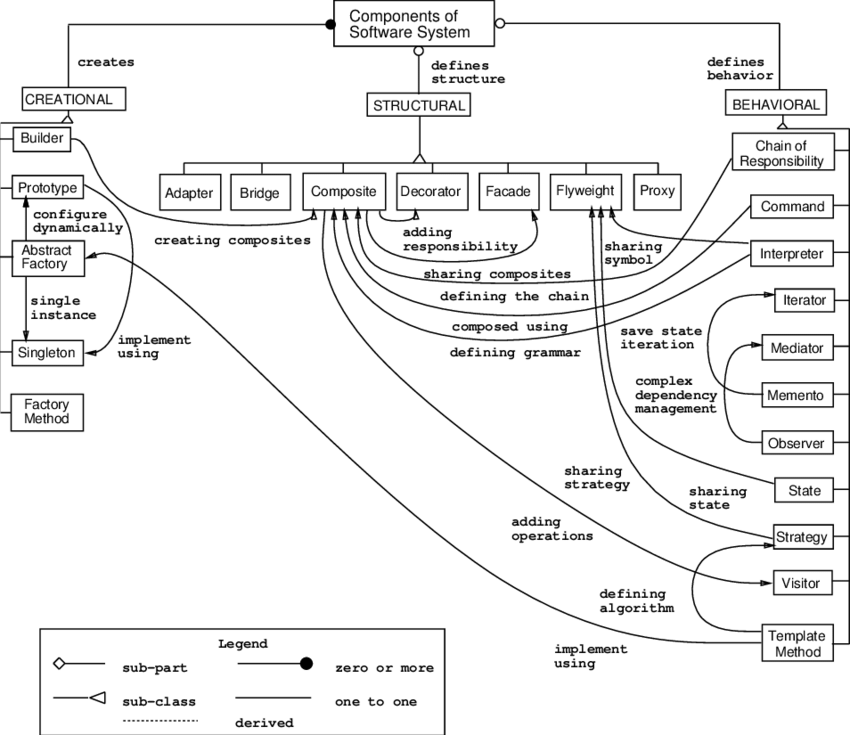
\includegraphics[scale=0.5]{image/dp3.png}  
\end{center}
Phía trên là sơ bộ các mối quan hệ giữa các Patterns với nhau. Có thể dễ dàng thấy các Patterns này đếu được phát triển tử các Pattern khác, nên trong tương lai có khả năng sẽ có thể xuất hiện thêm nhiều Pattern tiện lợi và hiện đại hơn.
